\documentclass[10pt, conference, letterpaper]{IEEEtran}
\usepackage{cite}
\usepackage{xcolor,soul,framed}
\usepackage{amsmath,amsthm,amssymb,amsfonts}
\usepackage{algorithmic}
\usepackage{graphicx}
\usepackage{color, soul}
\usepackage{algorithm, algorithmic}
\usepackage[utf8]{inputenc}
\usepackage[english]{babel}
\usepackage{mathtools}
\graphicspath{ {./images/} }

%---------------------------------------------------------------%
\newtheorem{definition}{Denifition}
\newtheorem{assumption}{Assumption}
\newtheorem{problem}{Problem}
\newtheorem{lemma}{Lemma}
\newtheorem{corollary}{Corollary}
\newtheorem{example}{Example}
\newcommand{\eq}{=}
\newcommand{\domZ}{\mathbb{Z}_{*}}
\newcommand{\vecOne}{\mathbf{1}}
\newcommand{\ind}{\mathbf{I}}
\newcommand{\mat}{\mathbf}
\newcommand{\define}{\triangleq}
\renewcommand{\vec}{\mathbf}
\DeclarePairedDelimiter\set\{\}
% \DeclarePairedDelimiter\set\bigg(\bigg)
%---------------------------------------------------------------%
\newcommand{\apSet}{\mathcal{K}}
\newcommand{\esSet}{\mathcal{M}}
\newcommand{\jSet}{\mathcal{J}}
\newcommand{\wSet}{\mathcal{W}}
\newcommand{\uSet}{\mathcal{U}}
\newcommand{\cSet}{\mathcal{C}}
\newcommand{\Stat}{\mathbf{S}}
\newcommand{\Obsv}{\mathcal{X}}
\newcommand{\Policy}{\mathbf{\Omega}}
%---------------------------------------------------------------%

\begin{document}

    %=============================== TITLE ===============================%
    \title{
        Meet-in-Future: Distributed Online Job Dispatching with Obsolete Information in Edge Computing System
    }
    \author{
        \IEEEauthorblockN{Yuncong Hong$^{*\dagger}$}
        \IEEEauthorblockA{
            $*$Southern University of Science and Technology, P.R. China,
            $\dagger$The University of Hong Kong, Hong Kong,\\
            $\ddagger$University of Science and Technology of China, P.R. China
        }
    }
    \maketitle

    %============================== ABSTRACT ==============================%
    \begin{abstract}
        \label{sec:abstract}
        Edge computing is believed to be the solid solution for time-sensitive big data real-time calculation. The cooperation among edge servers in the same coalition usually causes ineffective task scheduling due to obsolete information sharing, which is hard to tackle even with extra centralized agent design. In this work, we formulate the problem with job dispatching in distributed Edge Computing system, and identify the difficulty exists in cooperation between AP nodes (Access Points) and ES nodes (Edge Servers) with delayed information. We design the broadcast information in the system and formulate the corresponding problem into a MDP problem. The value function approximation and \st{one-step policy iteration method is adopted to obtain a sub-optimal dispatching policy whose performance can be bounded analytically}.
    \end{abstract}

    % \begin{IEEEkeywords}
    %     Edge Computing, Job Dispatch, Delayed Information, Collective Observability, Distributed Multi-agent MDP
    % \end{IEEEkeywords}

    %============================ INTRODUCTION ============================%
    \begin{section}{INTRODUCTION}
        \label{sec:introduction}
        Our claims:
        \begin{itemize}
            \item Related works on scheduling in edge computing, mostly with centralized agent to apply action and seldomly take delayed information impact into consideration;
            \item Edge Server, Access Point, User Equipment; layered structure where decision is made distributedly on AP nodes and computation is carried out on ESs; The AP-ES fully connected structure is reasonable, for example C-RAN to separate communication and computation 
            \item We identify the delayed system information is un-acceptable for explosion \emph{delay-sensitive jobs} in edge computing, and it's hard to establish cooperation among AP nodes because of obsolete information;
            \item information sharing for cooperation is designed via (aligned) broadcast, job dispatch decision should be made immediately based on the previous collective information;
        \end{itemize}

        Our contributions:
        \begin{itemize}
            \item identify a instant job dispatch fully-distributed cooperative way, and avoid the centralized agent design;
            \item identify the uploading process may affect the heuristic greedy algorithm performance; identify the delay-information affected decision making;
            \item propose a global consensus state method to formulate the MDP problem (we use MDP definition in \cite{sutton1998introduction});
            \item adopt value function approximation to reduce the traditional algorithm complexity, and come up with distributed online learning algorithm;
        \end{itemize}

        Related works:
        \begin{itemize}
            \item The earliest related works we find is \cite{ref-01} (cited 167 times). In this work, the single agent is assumed not able to observe the global state, and thus they need communication to establish cooperation by sharing \emph{information}. The agent considers communication as extra action to synchronize the states and thus incurs extra cost. \\
            However, the communication is without delay, and converted into POMDP problem.
            \item The other work \cite{ref-02} considers continuous state observation with constant or stochastic delay with single agent. \\
            However, 
        \end{itemize}

    \end{section}

    %============================ SYSTEM MODEL ============================%
    \begin{section}{SYSTEM MODEL}
        \label{sec:model}
        \begin{subsection}{Network Model}
            The network topology of the MEC system considered is illustrated in Fig. \ref{fig:system}, which is composed of three elements. The access point (AP) provides network access to all the user equipment (UE) connected and accept the computation jobs released from UEs. The AP itself is assumed with no computation capability, and then dispatches the jobs to edge servers (ES) following the policy. The ES would complete the computation jobs in a fairness way that takes no bias on any AP nodes. The network topology between AP cluster and ES cluster is assumed fully connected so that AP could access any edge servers in this coalition with communication cost.

            We adopt \emph{timeslot} lasting for $\kappa$ seconds as the minimum time slice in the system, which is indexed with $t$. The dispatching and scheduling decision on AP and ES side respectively are all applied based on this timing. Moreover, the information sharing in this coalition is designed via broadcast to achieve decentralized cooperation among AP nodes.
            The periodic broadcast is called \emph{aligned broadcast}, where all the AP and ES nodes start to broadcast at the start of the same timeslot, and repeat broadcasting with the same interval as $T_B$ time slots. More specifically, the AP nodes should broadcast their system information at the broadcast point to the other AP nodes, and the ES nodes should also broadcast their information to all AP nodes. \hl{The precision of aligned broadcast could be guaranteed by timely synchronization protocol or with GPS device, which is not the main focus in our discussion.}
            \begin{figure}[ht]
                \centering
                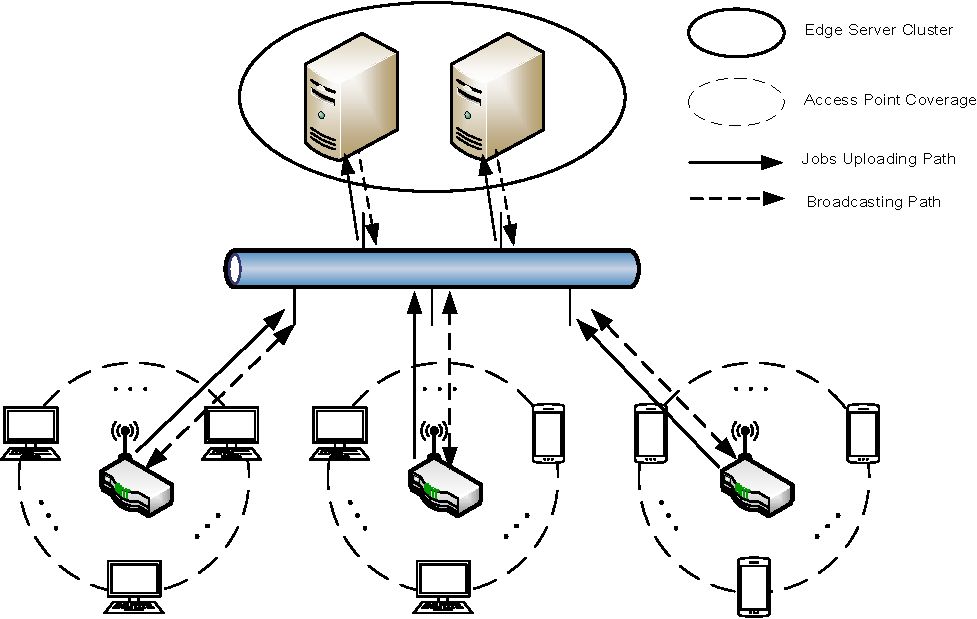
\includegraphics[width=0.45\textwidth, trim={0.5cm 0.5cm 0.5cm 0.5cm}, clip]{system-model.pdf}
                \caption{The Illustration of MEC System Model}
                \label{fig:system}
            \end{figure}

            Now we give the formal definition of the network illustration. Let $\mathcal{K} \triangleq \set{1,\dots,K}$ and $\mathcal{M} \triangleq \set{1,\dots,M}$ denote the set of AP nodes and set of ES nodes in the MEC system respectively. The jobs released from UEs connected with $k$-th AP $\forall k\in\apSet$ is denoted as the \emph{job arrival process} and follows the assumption as:
            \begin{assumption}
                (Job Arrival Process at $k$-th AP).
                We assume that the job arrival process $A_k(t)$ for $k$-th AP is i.i.d over the $t$-th timeslot and with Bernoulli distribution $A_k(t) \sim Bernoulli(\lambda_k)$.  According to Poisson Limit Theorem, we identify the arrival process as memory-less exponential process and with average arrival rate $\mathbb{E}[A_k(t)] = \lambda_k$.
                This assumption implies that there will be at most one job arrives AP in one timeslot from all the UEs connected.
            \end{assumption}

            There are two main communication process with AP and ES nodes engaged based on the network topology elaborated above. We assume the communication latency is rather deterministic between two nodes and assign the delay time directly w.r.t transmission content for convenience.

            There are two communication process illustrated in the edge computing system which are applied on different time scale.
            
            The first one is \emph{uploading process} where AP dispatches jobs to corresponding ESs and applied on each timeslot. The uploading time is {\color{red}job-independent} and deterministic for all kinds of jobs on AP-ES link, which is denoted as $T^{prop}_{k,m}$ for from $k$-th AP to $m$-th ES, and the uploading time always lasts for integer timeslots. \emph{Parallel uploading} is enabled on AP to alleviate the cost caused by serially uploading process. As the arrival process and uploading time is bounded, there will be at most $\lambda_k \cdot \max_m(T^{prop}_{k,m})$ jobs in transmission on $k$-th AP which results into finite bandwidth requirement.
            
            The other one is \emph{broadcast process} where AP nodes obtain the information about the global system state and applied on broadcast interval scale. We denote each broadcast time slot, called \emph{broadcast point}, as $t_i$ for $i$-th broadcast where,
            \begin{align}
                t_i = i T_B, i=0,1,2\dots
            \end{align} 
            Let $d^{(AP)}_{k,k'}$ denotes the broadcast delay from $k'$-th AP to $k$-th AP ($\forall k,k'\in\apSet$) w.r.t. the last broadcast point; let $d^{(ES)}_{k,m}$ denotes the broadcast delay from $m$-th ES to $k$-th AP ($\forall m\in\esSet$). It's reasonable to assume that the broadcast interval is always larger than broadcast delay, i.e. $T_B > d^{(AP)}_{k,k'}, T_B > d^{(ES)}_{k,m}$. To denote the timeslot where $k$-th AP could receive all the broadcast information thus obtain global state view, we come up with the concept called \emph{consensus delay} for AP nodes as:
            \begin{definition}
                (Consensus Delay).
                \begin{align}
                    \hat{d}_k = \max(\set{d^{(AP)}_{k,k'}|\forall k,k'\in\apSet}, \set{d^{(ES)}_{k,m}|\forall k\in\apSet,m\in\esSet}),
                \end{align}
                where $d^{(AP)}_{k,k} \equiv 0$. \hl{The consensus delay is the time after last broadcast point where $k$-th AP could obtain the global state view and come to consensus with the complete information.}
            \end{definition}
        \end{subsection}

        \begin{subsection}{Computation Model}
            For computation process on edge servers, we adopt \emph{unrelated machines} assumption in \cite{tan-online}, where the job processing time on different servers are machine dependent and variant of resource or VM (virtual machine) constraints.
            The maximum processing time in this system is bounded with $L_C$.
            The job space is denoted as $\jSet$ and its cardinality is denoted as $|\jSet|=(L_C)^M$ for all possible job processing time on all $M$ ES nodes.
            Moreover, we have the mapping function $f:\jSet \to \domZ^M$ to store process time vector for job in jobs space.
            Additionally, the jobs arrival process on each AP node has the same distribution over job set $\jSet$ which is denoted as: $p_j \define \Pr(j\in\jSet)$.
            
            We assume the scheduling policy on all the servers as following:
            \begin{assumption}
                (Scheduling Policy).
                All the edge servers adopt \emph{FCFS} (First-Come-First-Serve) as job scheduling policy, i.e. the job earlier arrives at the server would get served earlier. And we note that the arrival order is not only determined by job arrives at the access point, but also related with the uploading latency.
            \end{assumption}
        \end{subsection}

        \begin{subsection}{Job Dispatching Model}
            The job dispatching process on each job is composed of three stages: dispatching decision making, uploading, and waiting for service. According to the communication model and computing model illustrated above, there would be accumulated job set on AP and ES nodes respectively.

            As the transition is initialized by \emph{dispatching decision} over arrival job in $t$-th timeslot on each AP, we give the definition for decision action space denotation here:
            \begin{definition}
                (Dispatching Action Space).
                The dispatching action space is applied job-wise in the waiting job set denoted as $a: \jSet \times \set{1,\dots,M}$, where $(j, m)$ denotes the action that $j$-th job should be uploaded to $m$-th ES.
            \end{definition}

            \begin{itemize}
                \item Two time scale; dispatching process is carried out on each timeslot based on dispatching decision, but the scheduling decision is carried out on each broadcast point;
                \item Separate uploading and computing process; the uploaded jobs on ES nodes in this broadcast interval, would join computing with scheduling policy in next broadcast interval; \hl{(to alleviate curse of dimensionality in problem formulation)}
                \item We have the denotation on $i$-th broadcast point with broadcast time scale;
                    \begin{itemize}
                        \item for $k$-th AP ($\forall k\in\apSet$), it has $\set{u_{k,m}(i)|\forall m\in\esSet}$ series to denote uploading process, where $u_{k,m}(i)$ denotes the number of jobs still in uploading at time $t_i$;
                        \item for $m$-th ES ($\forall m\in\esSet$), it has $Q_m(i)$ to denote the FIFO queue and each element $e \in Q_m(i)$ denotes the remaining processing time for that job;
                    \end{itemize}
            \end{itemize}

            Then we have the denotation of system observation on $i$-th broadcast point as:
            \begin{align}
                \Obsv(t) \define \{ \set{u_{k,m}(t)|\forall k\in\apSet,m\in\esSet}, \set{Q_m(t)|\forall m\in\esSet} \}
            \end{align}
        \end{subsection}
    \end{section}

    %============================ FORMULATION =============================%
    \begin{section}{FORMULATION}
        \label{sec:formulation}
        In this section, we formulate the standard MDP problem based on the MEC system elaborated above. The optimization problem will be formulated globally on dispatching decisions on AP nodes, but applied fully distributed on each AP with broadcast design to share information.

        \begin{subsection}{System State and Scheduling Policy}
            we firstly clarify the broadcast information from AP nodes and ES nodes.
            The observation at $\tau$-th broadcast, $\Obsv(T_\tau)$ is denoted as $\Obsv_\tau$ for short. The broadcast information is based on $\Obsv_\tau$ as:
            \begin{definition}(Broadcast Information).
                The $k$-th AP would broadcast all the job set information at $T_\tau$ as $\wSet_{k}(T_\tau), \bigcup\limits_{m\in\esSet}\uSet_{k,m}(T_\tau)$.
                Thus the composed broadcast information at $T_\tau$ is:
                \begin{itemize}
                    \item System observation at $T_\tau$ timeslot, $\Obsv_\tau$;
                \end{itemize}
            \end{definition}

            This broadcast information is also called \emph{global consensus} in Fig. \ref{fig:br-trans} \hl{(need to modify the state denotation in figure)} that $k$-th AP would only obtain the broadcast information completely after the \emph{consensus delay} $\hat{d}_{k}$ w.r.t to the last broadcast point. The system state of the formulated MDP problem is on the global consensus but locally computed at each AP nodes, given as following:
            \begin{definition}(System State).
                At the $\tau$-th broadcast on broadcast point $T_\tau$, the global state for all AP nodes is denoted as: $\Stat_\tau = (\Obsv_{\tau}, \Obsv_{\tau-1}, \vec{n}_\tau), (\tau=1,2,\dots)$.
                More specifically, the $k$-th AP nodes would come up with this global state consensus only after $\hat{d}_k$ timeslots, and it adopt policy based on the obsolete information.
            \end{definition}
            \begin{figure}[ht]
                \centering
                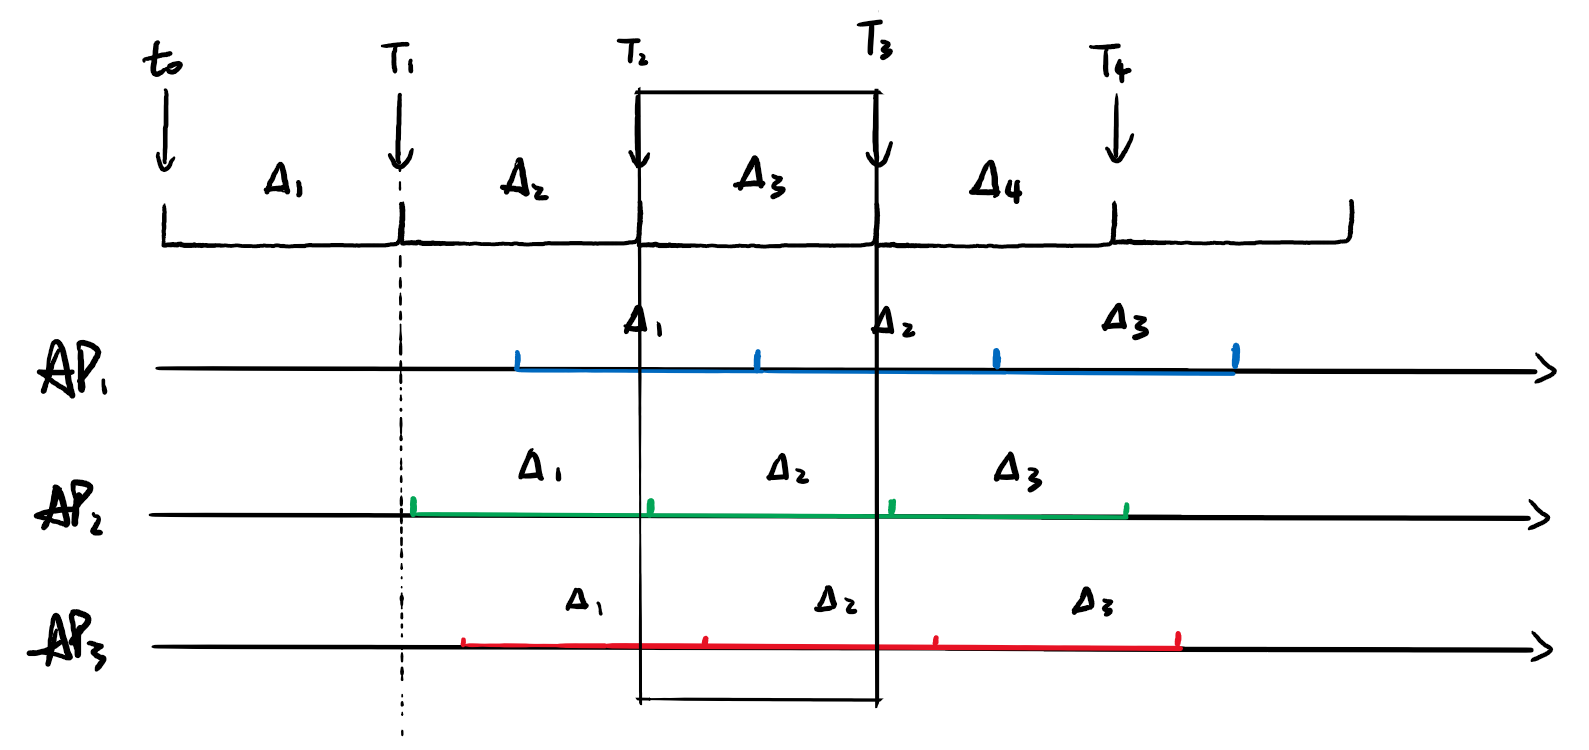
\includegraphics[width=0.45\textwidth]{broadcast-trans.png}
                \caption{Global Consensus and Transition with Delayed Action}
                \label{fig:br-trans}
            \end{figure}

            The dispatching policy $\vec{\Omega}(\Stat_\tau)$ is actually composed of all AP nodes based on obsolete information $\Obsv_{\tau-1}$ and the updated information $\Obsv_{\tau}$ after the consensus delay $\hat{d}_k$ respectively. The composed policy over job-wise action space $\vec{a}$ is defined as following:
            \begin{definition}(Compounded Dispatching Policy).
                The compounded dispatching policy over $\Stat\tau$ is defined as $\Policy(\Stat_\tau)$ which is composed of the local policy $\Omega_k(\Stat_\tau), \forall k\in\apSet$ as:
                \begin{align}
                    \vec{\Omega}(\Stat_\tau) \triangleq [\Omega_1(\Stat_\tau), \dots, \Omega_K(\Stat_\tau)]
                \end{align}
                More specifically, $\Omega_k(\Stat_\tau)$ is composed of two-stage policy with $\tilde{\Omega}_k(\Obsv_{\tau-1})$ and $\tilde{\Omega}_k(\Obsv_{\tau})$ as:
                \begin{align}
                    \Omega_k(\Stat_\tau) = 
                    \begin{cases}
                        {\omega}_k(\Obsv_{\tau-1}), & 0 \leq \Delta{t} < \hat{d}_k
                        \\
                        {\omega}_k(\Obsv_{\tau}), & \hat{d}_k \leq \Delta{t} \leq T_B
                    \end{cases}
                \end{align}
                where $t\in[T_{\tau-1}, T_{\tau}] ,\Delta{t} \define t - T_{\tau-1}$; ${\omega}_k(\Obsv_\tau)$ denotes the dispatching policy, which is a mapping from $\Obsv_\tau$ to a probabilistic distribution over action space $\vec{a}$ for $k$-th node.
            \end{definition}

            As the state transition from $\Stat_{\tau}$ to $\Stat_{\tau+1}$ is driven by the compounded policy with the obsolete state $\Obsv_{\tau-1}$, and the updated state $\Obsv_{\tau}$ with delay.
        \end{subsection}

        \begin{subsection}{The Optimization Problem}
            The optimization target of our problem is to minimize the \emph{average response time} of all jobs, which is composed of waiting time on AP, uploading time, waiting time on ES and service time on ES. According to \emph{Little's Law}, the average time over all the jobs is equally as number in system accumulation in each timeslot. The cost function is:
            \begin{align}
                g\bigg(\Stat_\tau, \Policy(\Stat_{\tau-1})\bigg) \define \sum_{k\in\apSet}\sum_{m\in\esSet} u_{k,m}(\tau) + \sum_{m\in\esSet}|Q_m(\tau)| 
            \end{align}
            which is actually deterministic with the $\tau$-th broadcast information.
            Our distributed optimization problem definition is given as following:
            \begin{problem}
                (Distributed Cooperative Job Dispatching Problem).
                \begin{gather}
                    \min_{\Policy} \lim_{T \to \infty}
                        \mathbb{E}_{\Policy, \{A_k(t)|\forall k\in\apSet\}}
                            [\sum_{\tau=1}^{T} \gamma^{\tau-1} g(\Stat_\tau, \Policy(\Stat_{\tau-1}))|\Stat_1]
                \end{gather}
            \end{problem}

            According to \cite{sutton1998introduction}, the above problem could be solved by the following \emph{Bellman's equation}:
            \begin{align}
                V(\Stat_{\tau}) =& g(\Stat_\tau) +\gamma \min_{\Policy(\Stat_\tau)} \sum_{\Stat_{\tau+1}} \Pr\{\Stat_{\tau+1}|\Stat_{\tau}, \Policy(\Stat_\tau)\} V(\Stat_{\tau+1})
                \nonumber\\
                =& g(\Stat_\tau) +\gamma \min_{\Policy(\Stat_\tau)} \sum_{\Stat_{\tau+1}} \Pr\{\Stat_{\tau+1}|\Stat_{\tau}, \Policy(\Stat_\tau)\}
                \nonumber\\
               & \cdot [\sum_{k\in\apSet} {W}^{(k)}(\tilde{S}^{(k)}_{\tau+1}) + \sum_{m\in\esSet} {W}^{(m)}(\tilde{S}^{(m)}_{\tau+1})],
            \end{align}
            where $W^{(k)}=\mathbb{E}\{\}, \forall k\in\apSet$, and $W^{(m)}=\mathbb{E}\{\}, \forall m\in\esSet$

            There are totally $(K+1)$ transition matrix in $[T_{\tau}, T_{\tau+1})$ w.r.t. $\hat{d}_k$ and denoted as $\mat{P}^{\Delta{t}_k}$ in $\Delta{t}_k$ interval for all $k\in[0,1,\dots,K]$.
        \end{subsection}
    \end{section}

    %============================= ALGORITHM ==============================%
    \begin{section}{LOW-COMPLEXITY SOLUTION}
        \label{sec:algorithm}
        As the formulated problem above is of infinite states and the action space would be exponentially expanded with respect to number AP and ES nodes, we could not use traditional \emph{policy iteration} or \emph{value iteration} algorithm \cite{sutton1998introduction} for unacceptable computational complexity. To alleviate curse of dimensionality, we take one baseline policy to approximate the value function as $\tilde{V}(T_t)$ and carry out one-step iteration to come up with a better value function approximation.
        \hl{Traditional value iteration is intractable due to the following reasons: (1) the number of active devices is not fixed and the state space grows exponentially with the increasing number of active devices; (2) the spaces of small-scale fading and path-loss are continuous.}

        \begin{subsection}{Baseline Policy}
            \begin{problem}
                (Fixed FCFS Optimization).
                \begin{itemize}
                    \item no waiting stage;
                    \item locally greedy uploading;
                    \item FCFS scheduling (?);
                \end{itemize}
            \end{problem}

            \begin{definition}
                (Job Arrival Process at $n$-th ES).
            \end{definition}

            At last, we collect the cost according to the definition in our MDP problem but with respect to our approximate algorithm.
            \begin{align}
                & \tilde{V}^{\pi}(T_t)
                \nonumber%\\
                = E_{\pi} \{ \tilde{C}_{t} + \gamma \tilde{C}_{t+1} + \gamma^2 \tilde{C}_{t+2} + \dots |S_{t-1}=s \}
                % \nonumber\\
                % = & \sum_{k=0}^{\infty} \gamma^{k} \sum_{t'=kT^{br}+1}^{(k+1)T^{br}} \sum_{s'} \tilde{P}^{t'}_{s,s'} \times |s'|
            \end{align}
            % where $\tilde{P}_{s,s'}$ is fixed under the given policy $\vec{\beta}_{\pi}$.
        \end{subsection}

        \begin{subsection}{The Distributed Algorithm}
            Then we introduce the one-step iteration algorithm in this section:
            % [\IF, \ENDIF], [\FOR, \TO, \ENDFOR], [\WHILE, \ENDWHILE], \STATE, \AND, \TRUE
            \begin{algorithm}[H]
                \caption{Distributed Algorithm for $k$-th AP}
                \begin{algorithmic}
                    \WHILE{\TRUE}
                        \STATE (in progress...)
                        % \FOR{$k \in \mathcal{K}$}
                        %     \STATE fix policy $\vec{\Omega}^{(k)}(t) \forall k' \neq k$
                        % \ENDFOR
                    \ENDWHILE
                \end{algorithmic}
            \end{algorithm}
        \end{subsection}
        
    \end{section}

    %============================ EVALUATION ==============================%
    \begin{section}{EVALUATION}
        \label{sec:evaluation}
        (in progress)
    \end{section}

    %============================= CONCLUSION =============================%
    \begin{section}{CONCLUTION}
        \label{sec:conclusion}
        The future work to mention:
        \begin{itemize}
            \item non-aligned broadcast
            \item broadcast failure
            \item randomized broadcast delay
        \end{itemize}
    \end{section}

    %============================== REFERENCE =============================%
    \bibliographystyle{IEEEtran}
    \bibliography{main.bib}
\end{document}